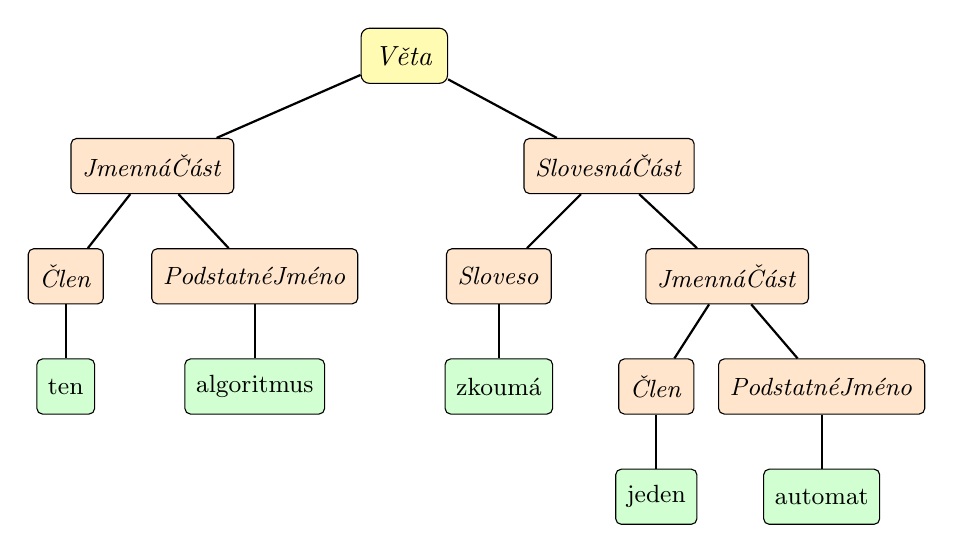
\begin{tikzpicture}[
    vet/.style={draw,rounded corners=3pt,fill=yellow!30,
        minimum height=7mm,inner xsep=5pt},
    net/.style={draw,rounded corners=2pt,fill=orange!20,
        minimum height=7mm,inner xsep=4pt,font=\small},
    term/.style={draw,rounded corners=2pt,fill=green!18,
        minimum height=7mm,inner xsep=4pt,font=\small}
]
    \node[vet] (veta) at (0,0) {\textit{Věta}};

    \node[net] (jm1) at (-3.2,-1.4) {\textit{JmennáČást}};
    \node[net] (slc) at (2.6,-1.4) {\textit{SlovesnáČást}};

    \node[net] (cl1) at (-4.3,-2.8) {\textit{Člen}};
    \node[net] (pj1) at (-1.9,-2.8) {\textit{PodstatnéJméno}};
    \node[net] (sl) at (1.2,-2.8) {\textit{Sloveso}};
    \node[net] (jm2) at (4.1,-2.8) {\textit{JmennáČást}};

    \node[term] (ten) at (-4.3,-4.2) {ten};
    \node[term] (alg) at (-1.9,-4.2) {algoritmus};
    \node[term] (zk) at (1.2,-4.2) {zkoumá};
    \node[net] (cl2) at (3.2,-4.2) {\textit{Člen}};
    \node[net] (pj2) at (5.3,-4.2) {\textit{PodstatnéJméno}};

    \node[term] (jeden) at (3.2,-5.6) {jeden};
    \node[term] (aut) at (5.3,-5.6) {automat};

    \foreach \x/\y in {veta/jm1,veta/slc,jm1/cl1,jm1/pj1,slc/sl,
        slc/jm2,cl1/ten,pj1/alg,sl/zk,jm2/cl2,jm2/pj2,cl2/jeden,pj2/aut}
        \draw[thick] (\x)--(\y);
\end{tikzpicture}
